%% fundamentals.tex
Machine learning uses mathematical functions to map an input to an output.
These functions usually extract patterns from the input data to build a relationship between input and output.
The term machine learning stems from the fact that we use \emph{machines} to correlate the input and the output to a function (i.e. to \emph{learn} a function) during a training period.
Deep learning is a sub-branch of machine learning and is considered state-of-the-art for many learning tasks, especially on high-dimensional data such as texts, audio recordings, 2D and 3D images, and videos.
Deep learning algorithms use neural networks that are heavily inspired by networks of neurons within the human brain.

Therefore, \secref{neurons} first briefly explains how biological neurons work and relates them to artificial neurons.
Next, \secref{ann} describes artificial neural networks that connect many artificial neurons.
In \secref{limitationsDL}, problems of such artificial neural networks are pointed out.
Next, \secref{biological_learning} describes some of the differences between deep learning and biological learning. Finally, \secref{neurocomputing} describes biologically more plausible learning methods that are investigated in the field of neurocomputing.
These last two sections are not important for understanding this thesis and can optionally be skipped. However, they are intended as a supplement for interested readers who want to get a better overview of the whole field.

\section{Biological Neurons}\seclbl{neurons}
\begin{figure}[h]
    \centering
    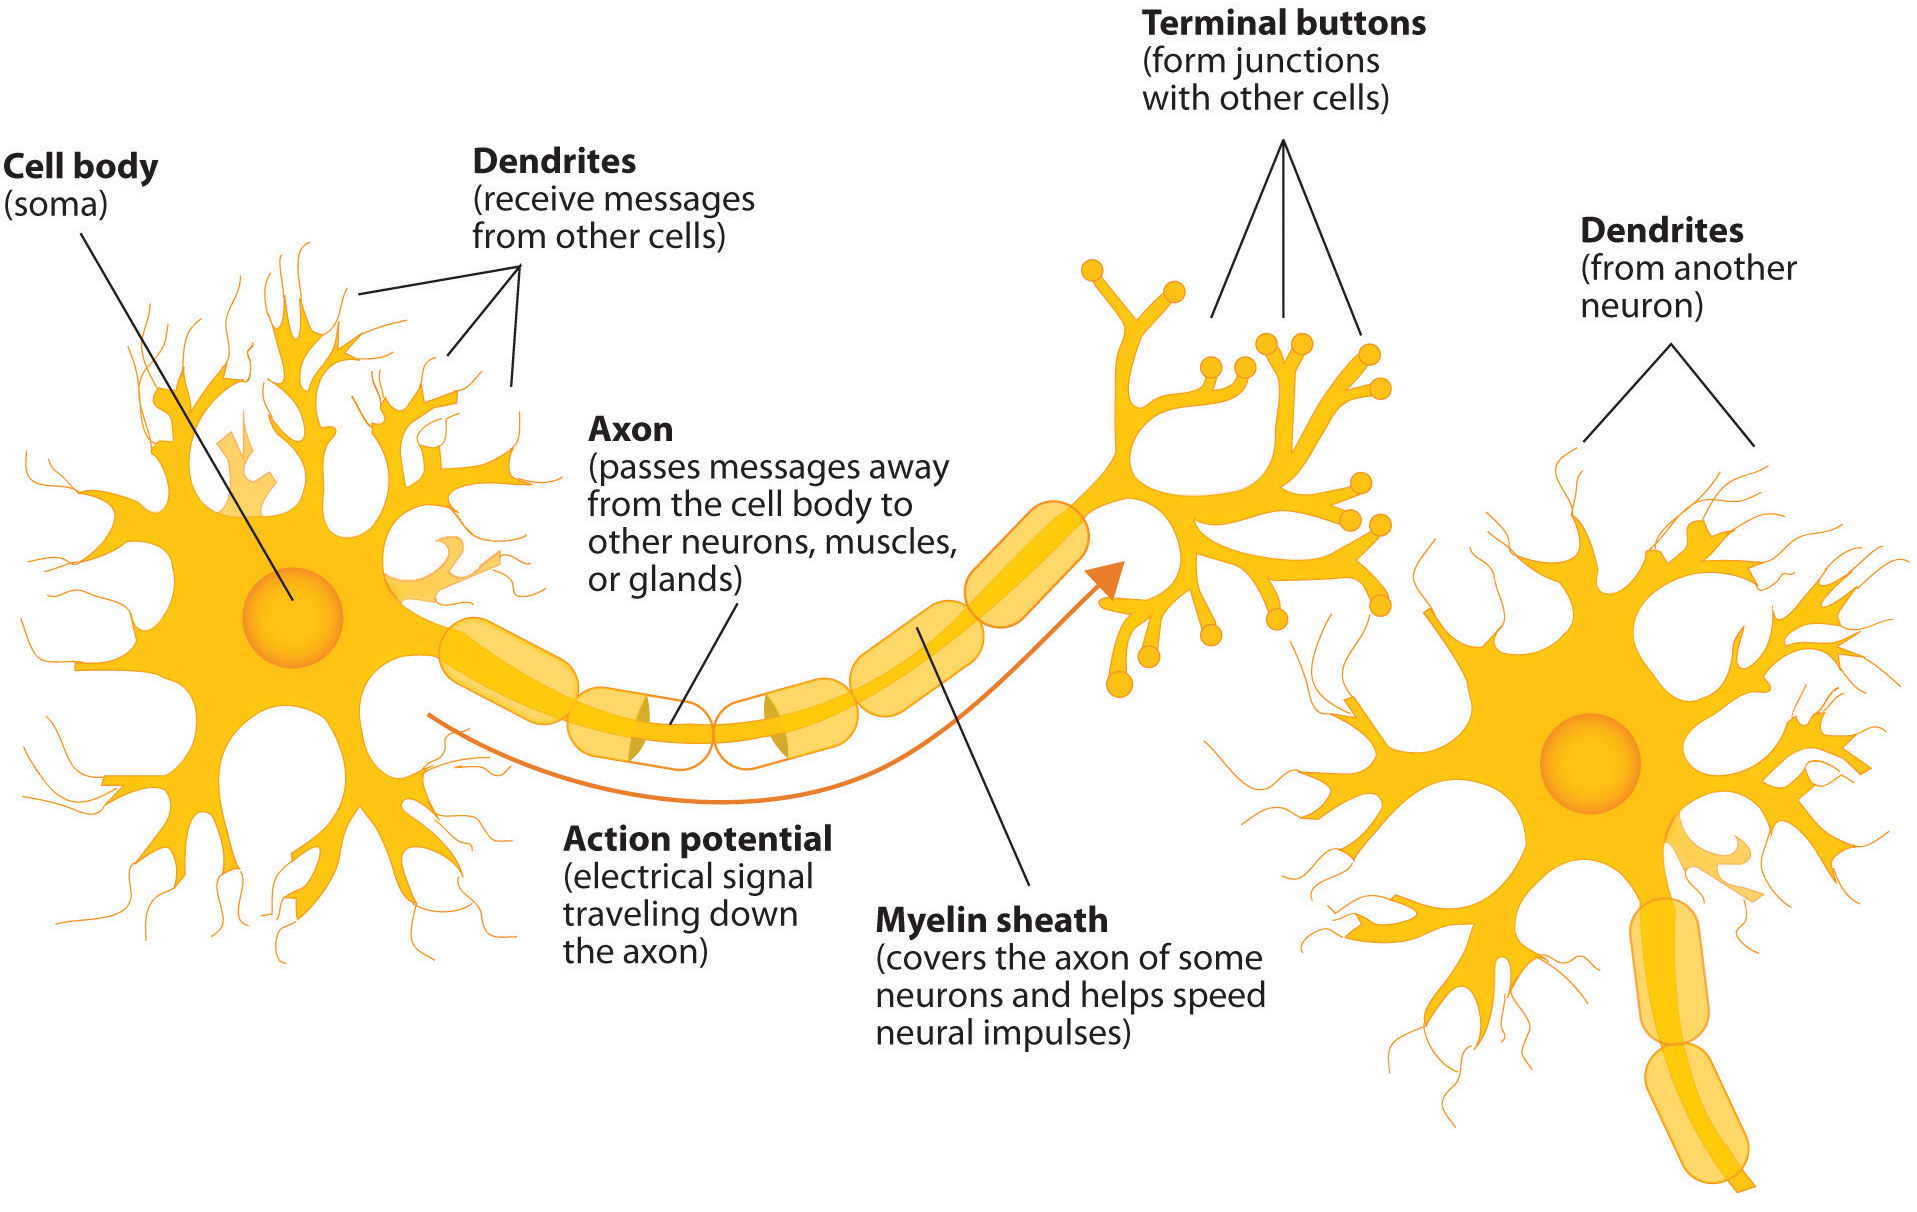
\includegraphics[width=0.99\textwidth]{components_of_neuron}
    \caption[Diagram of the components of a biological neuron]{A Diagram of the components of a biological neuron. The image is from \citeay{wiki_neuron}.}
    \figlbl{components_neuron}
\end{figure}

A biological neuron (c.f. \figref{components_neuron}) is a cell that communicates with other neurons through connections called synapses.
Communication takes place through precisely timed electrical pulses called spikes.
Biological neurons are electrically excitable by voltage changes across their membranes.
If the changes are significant enough within a short interval, the neuron generates a pulse called an action potential.
This action potential travels through the axon and activates synaptic connections.
Other neurons, connected through synapses, receive this signal.
The synaptic signal can be excitatory \sidecite{Takagi_2000} or inhibitory \sidecite{Coombs_Eccles_Fatt_1955}, making the post-synaptic neuron more or less likely to fire an action potential.
Biological neurons can be classified into sensory neurons, motor neurons, and interneurons.
Sensory neurons respond to external stimuli such as light or sound and send signals to the spinal cord or the brain.
Motor neurons receive brain and spinal cord signals to control muscles or organs.
Interneurons connect neurons within the same region of the brain or of the spinal cord.
Multiple connected neurons form a neural circuit.
The neural network in the brain is not static but changes through growth and reorganisation.
This process is referred to as neuroplasticity or neural plasticity \sidecite{Costandi_2016}.

Like a biological neuron, an artificial neuron is connected to other neurons.
Artificial neurons are usually organised in layers that forward signals sequentially.
Although the neurons in the first layer could be considered sensory neurons, the neurons in the last layer could be considered motor neurons, and the neurons in the middle layer could be considered interneurons, such a distinction makes less sense because the artificial neurons function similarly regardless of their layer except for the activation function.
Several variants for artificial neurons have been proposed in the literature. These variants are described in the following  \secref{ann}.
Like biological neurons, multiple artificial neurons are connected to artificial neural networks.


\section{Artificial Neural Networks}\seclbl{ann}
The idea for artificial neural networks (ANN) stems from biology and aims to capture the interaction of biological neurons with a mathematical model.
McCulloch and Pitts proposed the first model for a neuron that can be connected to other neurons in 1943 \sidecite{McCulloch_Pitts_1943}.
Similar to how a neuron of the human brain transmits electrical impulses through the nervous system, the artificial neuron of McCulloch and Pitts receives multiple input signals and transforms them into an output signal.
A neuron takes an input vector $\boldsymbol{x} = (x_1, ..., x_n)$ where $x_i \in \{0, 1\}$ and maps it to an output $\hat{y} \in \{0, 1\}$.
The mapping from the input to the output is done by using an aggregation function $g(\cdot)$ that sums up the input vector $\boldsymbol{x}$ and an activation function $f(\cdot)$ that outputs $1$ if the output of $g(\cdot)$ is bigger than a threshold $\theta$ and $0$ otherwise.
%
\begin{equation}\eqlbl{McCulloch_Pitts_agg}%
	z = g(\boldsymbol{x}) = g(x_1, ..., x_n) = \sum_{i=1}^{n}x_i\\
\end{equation}
%
\begin{equation}\eqlbl{McCulloch_Pitts_act}%
		\hat{y} = f(z) = \begin{cases}
      		1, & \text{if}\ z \geq \theta \\
      		0, & \text{otherwise}
    	\end{cases}
\end{equation}
%
In 1958, \sideciteay{Rosenblatt_1958} developed the Perceptron, which works with real numbers as input.
The input vector $\boldsymbol{x} \in \mathbb{R}^n$ is multiplied with a weight vector $\boldsymbol{w} \in \mathbb{R}^n$ with the same length $n$.
%
\begin{equation}\eqlbl{Perceptron_agg}%
	z = g(\boldsymbol{x}) = g(x_1, ..., x_n) = \sum_{i=1}^{n} w_i \cdot x_i\\
\end{equation}
%
The output $\hat{y} \in \{0, 1\}$ is similar to the McCulloch and Pitts neuron $1$ if the aggregated value is greater than a threshold $\theta$ and $0$ otherwise as described in \eqref{McCulloch_Pitts_act}. With real numbers as input, the equations \eqref*{Perceptron_agg} and \eqref*{McCulloch_Pitts_act} can be rewritten as
%
\begin{equation}\eqlbl{Perceptron}%
		\hat{y} =f(g(\boldsymbol{x})) = \begin{cases}
      		1, & \text{if}\ z - \theta \geq 0 \\
      		0, & \text{otherwise}
    	\end{cases}
\end{equation}
%
Later, the step-function \(f(\cdot)\) was replaced with other functions so that the output can also be a real number \(\hat{y} \in \mathbb{R}\). Often-used activation functions are
%
\begin{equation}\eqlbl{act_functions}%
	\begin{aligned}
		\text{Sigmoid: } & \sigma(z) = \frac{1}{1+\mathrm{e}^{-z}}\\
		\text{Rectified linear unit (ReLU): } & (z)^{+} = \max\{0, z\}\\
		\text{Hyperbolic tangent (tanh): }  & \tanh(z) = \frac{\mathrm{e}^{z}-\mathrm{e}^{-z}}{\mathrm{e}^{z}+\mathrm{e}^{-z}}
	\end{aligned}
\end{equation}
%
By convention, a positive bias $b$ is often used instead of the negative threshold $- \theta$, which leads to:
%
\begin{equation}\eqlbl{nn}%
	z = g(\boldsymbol{x}) = \boldsymbol{w} \cdot \boldsymbol{x} + b = \left( \sum_{i=1}^{n}w_i \cdot x_i \right) + b
\end{equation}
%
The neuron's output is calculated with the activation function of $z$:
%
\begin{equation}\eqlbl{nn2}%
	\hat{y} = f(z)
\end{equation}
%
So far, only the output of a single neuron has been discussed.
However, the brain consists of multiple neurons which are connected through synapses.
Therefore, also ANNs consist not only of one neuron but combine multiple neurons in a network. 
These neurons are organized in layers.
In the simplest case, all neurons from one layer are connected with all neurons of the subsequent layer. This is called a fully connected layer.
For a network with multiple neurons within one layer, the input $\boldsymbol{x}$ is fed into all neurons to obtain $\boldsymbol{\hat{y}}$.
If the layer has $k$ neurons, the output of the aggregation function becomes a vector $\boldsymbol{z} = (z_1, ..., z_k)$. The same applies to the output of the activation function $\boldsymbol{y} = (y_1, ..., y_k)$ and the bias $\boldsymbol{b} = (b_1, ..., b_k)$. The weight vector, on the other hand, becomes a matrix $\boldsymbol{W} = (\boldsymbol{w}_1, ..., \boldsymbol{w}_k)$. For a layer with multiple neurons, \eqref{nn} and \eqref{nn2} can be rewritten with matrix operations:
%
\begin{equation}\eqlbl{nn3}%
	\boldsymbol{z} = \boldsymbol{W} \cdot \boldsymbol{x} + \boldsymbol{b}
\end{equation}
\begin{equation}
	\hat{\boldsymbol{y}} = f(\boldsymbol{z})
\end{equation}
%
which is equal to
%
\begin{equation}\eqlbl{nn4}%
		\boldsymbol{z} = \begin{bmatrix}
			z_1\\
			z_2\\
			...\\
			z_k\\
		\end{bmatrix} = \begin{bmatrix}
			\boldsymbol{w}_1 \cdot \boldsymbol{x} + b_1\\
			\boldsymbol{w}_2 \cdot \boldsymbol{x} + b_2\\
			...\\
			\boldsymbol{w}_k \cdot \boldsymbol{x} + b_k\\
		\end{bmatrix} = \begin{bmatrix}
			\left( \sum_{i=1}^{n}w_{1i} \cdot x_i \right) + b_1\\
			\left( \sum_{i=1}^{n}w_{2i} \cdot x_i \right) + b_2\\
			...\\
			\left( \sum_{i=1}^{n}w_{ki} \cdot x_i \right) + b_k\\
		\end{bmatrix}
\end{equation}
\begin{equation}\eqlbl{nn5}%
		\hat{\boldsymbol{y}} = \begin{bmatrix}
			y_1 = f(z_1)\\
			y_2 = f(z_2)\\
			...\\
			y_k = f(z_k)\\
		\end{bmatrix}
\end{equation}
%

The universal approximation theorem\sidecite{Cybenko_1989} proves that a shallow network with one hidden layer (i.e. one layer between input and output layer) and enough neurons can approximate any mapping function between inputs and outputs.
However, very complex mapping functions may need too many neurons in the hidden layer.
Sequentially arranging multiple layers is much more efficient for approximating complex functions.
A sequential arrangement allows learning a hierarchy of features by dividing the mapping function over several successive processing steps.

In an MLP, the input \(\boldsymbol{x}\) is fed into the first layer, and each subsequent layer \(l\) uses the output of the previous layer \(l-1\) as input.
For a network with \(L\) layers, we denote the layer index as superscript square brackets, i.e. $(\cdot)^{[l]}$.
For example, the weights of layer $l$ are denoted as $\boldsymbol{W}^{[l]}$, the bias as \(\boldsymbol{b}^{[l]}\), the output of the aggregation function as \(\boldsymbol{z}^{[l]}\), and the output of the activation function as \(\boldsymbol{a}^{[l]}\).
The input in the first layer is the input data, i.e. $\boldsymbol{a}^{[0]} = \boldsymbol{x}$, and the output of the last layer is the model's prediction, i.e. $\boldsymbol{a}^{[L]} = \hat{\boldsymbol{y}}$. Thus, the mathematical model of an MLP is defined as

\begin{equation}\eqlbl{mlp}
		\boldsymbol{z}^{[l]} = \boldsymbol{W}^{[l]}\boldsymbol{a}^{[l-1]} + \boldsymbol{b}^{[l]}
\end{equation}
\begin{equation}\eqlbl{mlp2}
		\boldsymbol{a}^{[l]} = f({z}^{[l]})
\end{equation}

So far, only the forward pass used to calculate the output $\boldsymbol{\hat{y}}$ has been discussed.
However, the model output $\boldsymbol{\hat{y}}$ will only be close to the target output $\boldsymbol{y}$ if the weights $\boldsymbol{W}^{[l]}$ and biases $\boldsymbol{b}^{[l]}$ are properly defined in every layer $l$.
These parameters are learned during a training period.
The training can take place in a supervised, semi-supervised, self-supervised (sometimes also called unsupervised), or reinforcement learning setting.
In supervised learning, the output of the model $\boldsymbol{\hat{y}}$ is compared to a given target output $\boldsymbol{y}$.
On the other hand, unsupervised learning tries to find patterns in the input data $\boldsymbol{x}$ and cluster the samples into meaningful groups without using pre-defined target labels. Typically, the target $\boldsymbol{y}$ is derived from the data automatically (e.g. predict a masked part of the data); since the model creates the target by itself, this approach is also called self-supervised.
Semi-supervised learning is a hybrid approach of the aforementioned principles that combines a small amount of labelled data with a large amount of unlabelled data.
Lastly, reinforcement learning algorithms aim to maximize the reward that they receive from an environment based on some action they executed.

These learning principles have in common that a loss function (also called objective function) $\mathcal{L}(\cdot)$ can calculate a loss value based on the model output $\boldsymbol{\hat{y}}$ and the target output ${\hat{y}}$. For example, the mean square error (MSE) can be used for regression problems or the negative log-likelihood for classification problems.
The chosen loss function is minimized iteratively with stochastic gradient descent (SGD)\sidenote{there also exist other optimization algorithms such as SGD with momentum, RMSprop, or Adam \citep{Kingma2015AdamAM}} until the network converges to a (local) minima.
The idea behind stochastic gradient descent is to make use of the fact that the negative gradient of the loss value points to the direction of the steepest descent (i.e. in the direction where the loss becomes smaller).
Therefore, SGD updates the network parameters by taking a step of size $\eta$ toward their negative gradient:
%
\begin{equation}\eqlbl{sgd}
	\begin{aligned}
		\Delta \boldsymbol{W}^{[l]} = & -\eta \cdot \left( \nabla_{\boldsymbol{W}^{[l]}} \mathcal{L} \right)\\
		\boldsymbol{W}^{[l]} \coloneqq & \boldsymbol{W}^{[l]} + \Delta \boldsymbol{W}^{[l]}
	\end{aligned}
\end{equation}
%
and
%	
\begin{equation}\eqlbl{sgd2}	
	\begin{aligned}
		\Delta \boldsymbol{b}^{[l]} = & -\eta \cdot \left( \nabla_{\boldsymbol{b}^{[l]}} \mathcal{L} \right)\\
		\boldsymbol{b}^{[l]} \coloneqq & \boldsymbol{b}^{[l]} + \Delta \boldsymbol{b}^{[l]}
	\end{aligned}
\end{equation}
%
The term $\left( \nabla_{\boldsymbol{W}^{[l]}} \mathcal{L} \right)$ is the gradient of the weights \(\boldsymbol{W}^{[l]}\)  with respect to the loss $\mathcal{L}(\cdot)$ and the term $\left( \nabla_{\boldsymbol{b}^{[l]}} \mathcal{L} \right)$ is the gradient of the bias \(\boldsymbol{b}^{[l]}\)  with respect to $\mathcal{L}(\cdot)$.
The gradients of the weights can efficiently be calculated with an algorithm called backpropagation of error \sidecite{Rumelhart_Hinton_Williams_1986}, which is, in fact, just an intelligent implementation of the chain rule\sidenote{While a detailed discussion on backpropagation is out of scope for this thesis, we refer interested readers to the deep learning course by Andrew Ng \cite{Coursera}}.

One of the most critical design decisions in creating ANNs is how the neurons are connected.
So far, only the case where every neuron of one layer is connected to every neuron of the following layer (so-called fully connected layer) has been described. 
Besides such dense connections, there are several alternatives.
Since this work deals with the processing of visual scenes, the most well-known image-processing network architecture, namely Convolutional Neuronal Networks (CNN), is presented below. This architecture is also primarily used in this thesis. However, various alternative architectures exist for computer vision, such as Vision Transformer (ViT) \sidecite{Dosovitskiy_Beyer_Kolesnikov_Weissenborn_Zhai_Unterthiner_Dehghani_Minderer_Heigold_Gelly_2021} or MLP Mixer \sidecite{tolstikhin2021mlp}, which, however, would go beyond the scope of this introduction to deep learning.























\subsection{Convolutional Networks}\seclbl{cnns}
Convolutional Neural Networks (CNNs) are particularly useful for finding patterns in images but can also be used to analyze non-image data such as audio data or time series.
Similar to FCNs, a CNN is composed of an input layer, an output layer, and many hidden layers in between.
A typical CNN consists of subsequently connected convolutional layers and pooling layers.
Usually, an activation function is applied after each convolutional layer while no activation function is used after pooling layers.
Depending on the task, the last layers can be different, e.g. for image classification the last layers are often fully connected.

Convolutional layers use convolution filters or kernels that slide along input features and create translation-equivariant\sidenote{most CNNs apply downsampling operations to the input and are therefore not translation-invariant but translation-equivariant \cite{Mouton_Myburgh_Davel_2020}} responses known as feature maps \sidecite{Zhang_Itoh_Tanida_Ichioka_1990}.
The size of the filter, which is typically a \(3\times 3\) matrix, determines the size of the receptive field.
The filter is applied to an area of the input, with that area having the same size as the filter.
When applying the filter, the dot product is calculated between the input and the filter and then fed into an output array (i.e. the feature map).
Afterwards, the filter shifts by a stride, repeating the process until the entire input has been processed.
Since only the kernel have to be learned, convolutional layers consists of much less parameters than equivalently sized fully connected layers.
This process of re-using the same weights at different locations of the input is also known as parameter sharing.
As described earlier, multiple convolutional layer can follow on each other.
By doing so, CNNs become hierarchical as the later layers can see the pixels within the receptive fields of prior layers.

Pooling layers reduce the size of the input by conducting dimensionality reduction.
Similar to convolutional layers, a filter slides along the input.
However, this filter does not have any learned parameter but apply an aggregation function.
Usually, the filter either select the pixel with the highest value (max pooling) or calculates the average (average pooling) within the receptive field and forwards it to the output array.
Pooling layers usually discard a lot of information but help to reduce complexity and increase robustness.

In the last decades, various CNN architectures have been proposed, usually consisting of different combinations of CNN and pooling layer.
Further improvements have been achieved by using parallel paths of convolutional layers, batch normalization \sidecite{Ioffe_Szegedy_2015}, and skip connections\sidenote{skip connections skips some of the layers in the network and add the output of a layer to the input of a later layer}.
In this thesis I do not go into these specific architectures but provide some references to some well known architectures; LeNet \sidecite{Lecun_Bottou_Bengio_Haffner_1998}, AlexNet \sidecite{NIPS2012_c399862d}, VGGNet \sidecite{Simonyan_Zisserman_2015}, GoogLeNet \sidecite{Szegedy_Liu_Jia_Sermanet_Reed_Anguelov_Erhan_Vanhoucke_Rabinovich_2014}, ResNet \sidecite{He_Zhang_Ren_Sun_2016}, U-Net \sidecite{Ronneberger_Fischer_Brox_2015}, Mask R-CNN \sidecite{He_Gkioxari_Dollar_Girshick_2017}, SSD \sidecite{Liu_Anguelov_Erhan_Szegedy_Reed_Fu_Berg_2016}, and YOLO \sidecite{Redmon_Divvala_Girshick_Farhadi_2016}.

\subsubsection{Training of Convolutional Neural Networks}\seclbl{train_cnns}
CNNs can be used in various applications such as image recognition, video analysis, natural language processing, anomaly detection in time series and many others.
Since this thesis deals with better representations for visual scenes, this chapter is limited to the typical image analysis tasks; image classification, object detection, and image segmentation.
An overview of these tasks is shown in Figure \figref*{img_analysis_tasks}.
The goal of image classification is to predict an image-level label, i.e. to predict what object is in the image.
A classic example of this problem is predicting whether a cat or a dog is in a picture.
This is typically done for images that only contain one object.
With a multi-label classifier, however, it is also possible to predict whether none, one or several classes are present, i.e. whether a cat, a dog or both are present in the image.
With image classification it is unclear where in the image these objects are located.
Object detection provides a remedy.
The aim of object detection is not only to determine what is visible in the image but also where.
The position of the object is usually indicated by a bounding box (i.e. a rectangle).
Especially when there are several objects within a picture, it is helpful to know which object is where, e.g. that the cat is to the left of the dog.
For some applications, predicting the position with bounding boxes is not sufficient.
In this case, semantic segmentation is often used.
Semantic segmentation is the task where each pixel is classified (the image is divided into segments) which leads to a pixel-wise mask for each object in the image.
This gives us exact information about the shapes of the objects.

\begin{figure}[h]
    \centering
    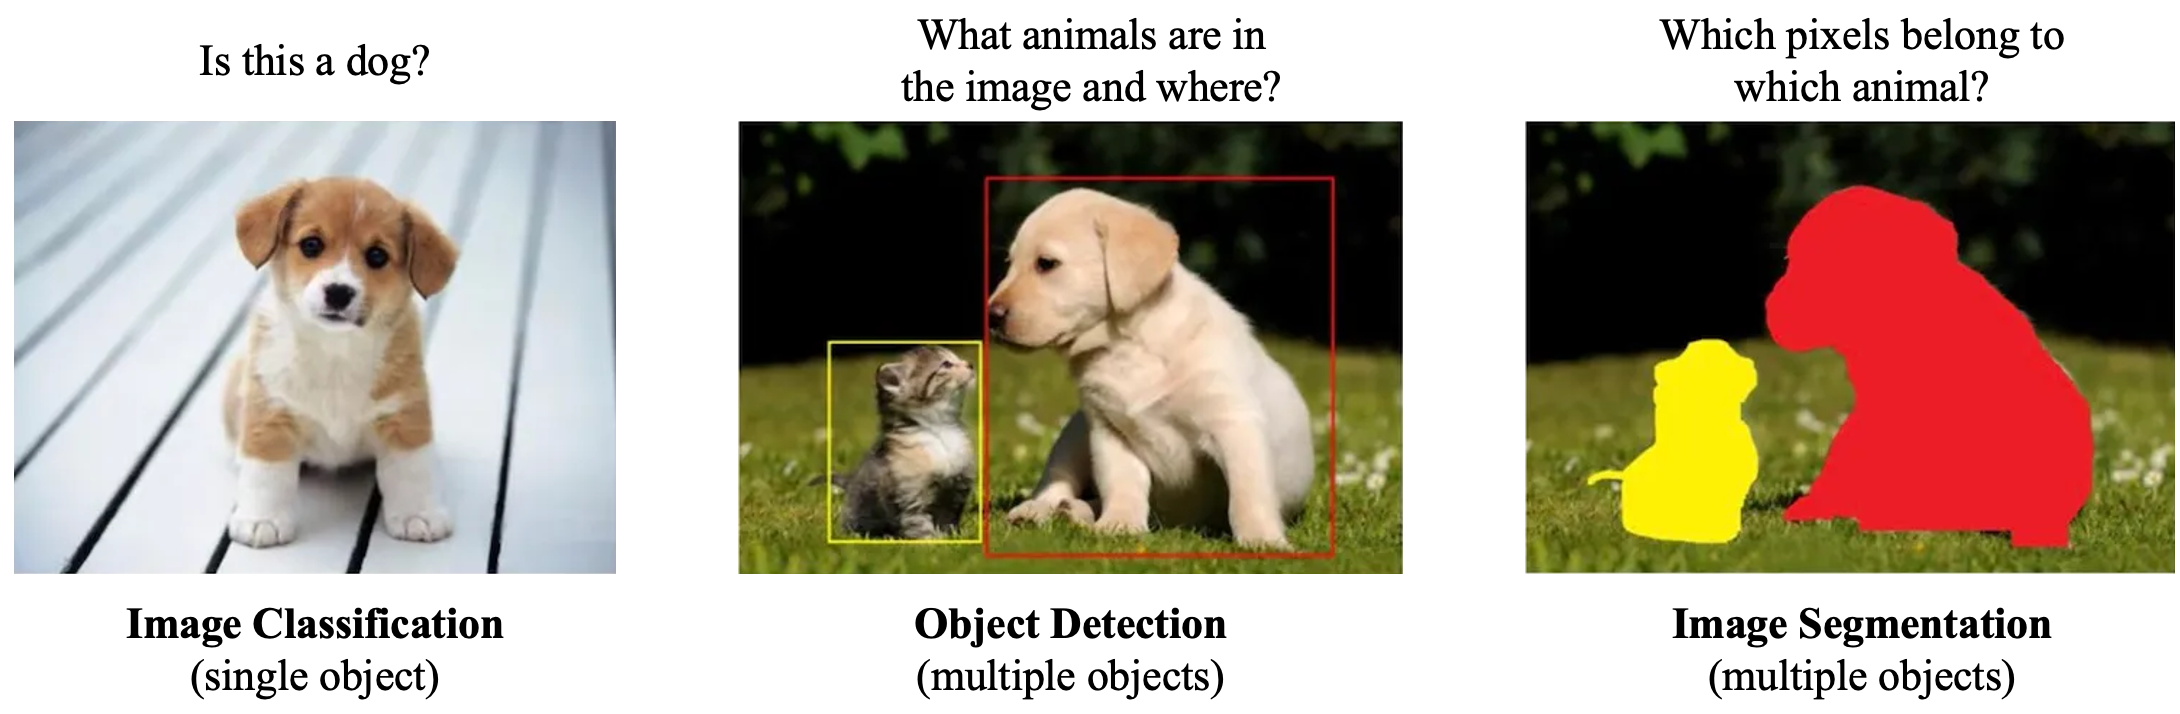
\includegraphics[width=0.99\textwidth]{image_analysis}
    \caption[Overview of different image analysis tasks]{Overview of different image analysis tasks. The image is taken from \citeay{venturebeat_img_analysis} and was slightly adapted.}
    \figlbl{img_analysis_tasks}
\end{figure}


Depending on the task, different kind of labels are required for supervised learning.
Image classification requires labels on image-level (i.e. one or multiple labels per image) \cite{Lecun_Bottou_Bengio_Haffner_1998, NIPS2012_c399862d, Simonyan_Zisserman_2015, Szegedy_Liu_Jia_Sermanet_Reed_Anguelov_Erhan_Vanhoucke_Rabinovich_2014, He_Zhang_Ren_Sun_2016}, object detection requires the coordinates of the bounding box \cite{Redmon_Divvala_Girshick_Farhadi_2016, Liu_Anguelov_Erhan_Szegedy_Reed_Fu_Berg_2016, He_Gkioxari_Dollar_Girshick_2017}, and semantic segmentation requires the labels on pixel-level \cite{Ronneberger_Fischer_Brox_2015, Wu_Zhang_Huang_Liang_Yu_2019} (i.e. each pixel has a label of an object or a label ``background'' for irrelevant pixels).

Besides supervised learning, there are various principles of learning with partial labels or without labels.
These techniques are called weakly-supervised or un-supervised learning and are well summarised in \sidecite{Simmler_Sager_Andermatt_Chavarriaga_Schilling_Rosenthal_Stadelmann_2021}.
Not only specific tasks can be learned, but also task-independent representations.
These representations are typically learned unsupervised\sidenote{also called self-supervised learning because the target labels are derived from the data itself} and can be used for one or several downstream tasks.
More details on visual representation learning are provided in Section \secref*{visual_rep_learning}.
Especially Autoencoders \sidecite{rumelhart1985learning} are explained in this section as they are applied in this thesis.


\section{Limitations}\seclbl{limitationsDL}
The rise of deep learning over the past decade has only been possible because of major technological advances in hardware.
Without the computational resources and the storage capacity of the systems created in the last decades no system could run today's algorithm.
Moreover, much of the progress of recent years was possible due to the improved hardware. 
Moore’s law \cite{Moore_2006} states that the number of transistors in a dense integrated circuit doubles about every two years and is the only known physical process following an exponential curve.
An analysis by OpenAI shows that since 2012 the amount of compute has even increasing exponentially with a doubling time  of \(3.4\) months \cite{OpenAI_compute}.
However, the exponential increase seems to come to an end since the size of transistors hit physical limitations.
It is assumed that Moore's law will end by around 2025 \sidecite{Kumar_2015}.
Besides the progress in the field and the development of new technology, deep learning models also became better because the number of parameters and the size of datasets grew exponentially.
Even the growth in the last five years is astonishing.
While the state-of-the-art language model from 2018 \sidecite{Peters_Neumann_Iyyer_Gardner_Clark_Lee_Zettlemoyer_2018} had around \(94\)M parameters, the state-of-the-art in 2020 \sidecite{NEURIPS2020_1457c0d6} already had \(175\)B parameters. Training such a model on a single V100 GPU would take about 355 years and cost about \(4.6\)M dollars \cite{Lambda_GPT3}.
A recent language model from Microsoft and Nvidia \sidecite{Shoeybi_Patwary_Puri_LeGresley_Casper_Catanzaro_2020} even has \(530\)B parameters.
Only a few institutions with massive resources are able to train such big models.
In general, inference on low-budget hardware such as smartphones or embedded hardware becomes prohibitive with the growing size of deep networks.
Even tough there exist techniques to shrink the model size after training such as quantization \cite{Wu_Judd_Zhang_Isaev_Micikevicius_2020}, model pruning \cite{Choudhary_Mishra_Goswami_Sarangapani_2020}, or model distillation \cite{Hinton_Vinyals_Dean_2015} it is questionable if making models bigger is the best way to develop intelligent systems.

Another major issue of deep learning systems is that they suffer from catastrophic forgetting.
If a model is trained on a specific task and afterwards trained (or fine-tuned) on another task, the model suffers a ``catastrophic'' drop in performance over the first task.
The reason for this effect is that the model during training on the second task adjusts the parameters learned during the first task and therefore ``forgets'' the learned mapping functions.
Just mixing all datasets or to learn all tasks in parallel in a current multi-task setup \cite{Zhang_Yang_2021} doesn't seem feasible to achieve some kind of general intelligence as this involves too many different unrelated tasks.
Catastrophic forgetting is also caused by the fact that learning is mostly done offline\sidenote{Offline in this context means that the model parameters are not adapted after training during inference time}.
Online learning \cite{Sahoo_Pham_Lu_Hoi_2017} and lifelong learning \cite{Parisi_Kemker_Part_Kanan_Wermter_2019} are currently hot research topics.
However, these methods have not yet been established.

Furthermore, there exists problems which may cannot be solved with the current principles used for deep learning.
First of all, it is questionable if deep learning models can achieve \emph{real} generalization\sidenote{Generalization refers to the ability of the model to adapt properly to previously unseen data from the same distribution}.
With enough data, can achieve generalization in the sense that the model can interpolate within the data distribution.
However, deep learning models fail to extrapolate.
For example, convolutional neural networks (CNNs) do not generalize to different viewpoints unless they are added to the training data \sidecite{Madan_Henry_Dozier_Ho_Bhandari_Sasaki_Durand_Pfister_Boix_2022}.

Second, deep learning is not able to learn abstract relationships in a few trials but requires many samples of it and is thus data hungry.\sidenote{Delme!!!}
Marcus Gary \sidecite{Marcus_2018} argues that if he tells that a ``schmister'' is a sister over the age of 10 but under the age of 21, humans can  immediately infer whether they or their best friends have any ``schmister''. However, modern DL systems lacks a mechanism for learning abstractions through explicit, verbal definition and require thousands or even more training samples.

Third, no DL model has been able to demonstrate causal reasoning in a generic way.
Deep learning models find correlations between the inputs and the outputs, but not the causation.
Other AI approaches such as hierarchical Bayesian computing or probabilistic graphical models are better at causal reasoning but cannot be well combined with deep learning models.

Lastly, deep learning models are to some extend too isolated since they have no embodiment and cannot interact with the world.
For example, the human body provides needs, goals, emotions, and gut feeling\sidenote{one could argue that the body is therefore even a co-processor of the brain}.
In current deep learning systems are emotions totally absent and the goals are set externally.
Deep Reinforcement Learning can be considered as a first step in the direction of dissolving this isolation, as they interact with a virtual environment. 
AI systems that interact with the real world do not work well so far.
Moravec's paradox \sidecite{Moravec_1995} states that ``it is comparatively easy to make computers exhibit adult level performance on intelligence tests or playing checkers, and difficult or impossible to give them the skills of a one-year-old when it comes to perception and mobility''.


\section{Biological Learning}\seclbl{biological_learning}
The human brain comprises many interconnected areas processing everything in parallel.
For example, Figure \figref{visual_cortext} illustrates the connections between different organizational units in the cerebral cortex which are responsible for vision.
It can be seen that these areas are connected in a rather complex structure.
\begin{figure}[h]
    \centering
    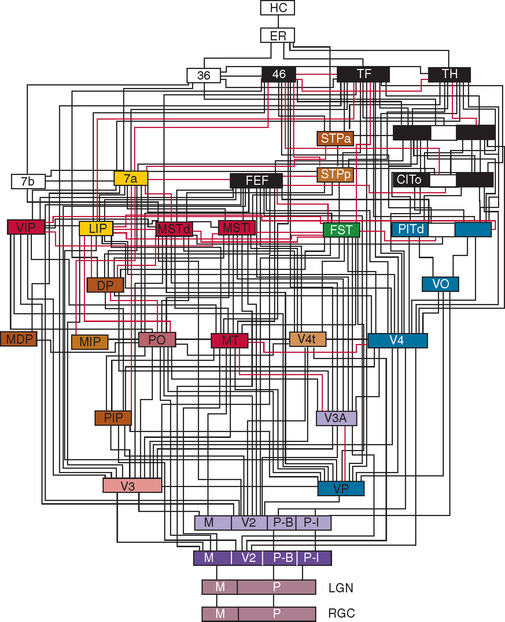
\includegraphics[width=0.99\textwidth]{felleman_visual_cortex}
    \caption[Organization of the visual system in the cerebral cortex]{The organization of the visual system in the cerebral cortex. The image is from \citeay{Felleman_Van_Essen_1991}.}
    \figlbl{visual_cortext}
\end{figure}
Deep learning architectures, on the other hand, are mostly unidirectional and the signal flows unidirectional from layer to layer\sidenote{Except for recurrent connections, skip-connections, or residual-connections}.
However, the choice of the architecture influences the how the model can learn the mapping function from input to output.
It could be that the complex structure of our brain comprises an inductive bias which was learned over time through evolution.

A learning system requires a mechanism that tells the system if something goes well or wrong so that it can learn from it.
This is called the \emph{credit assignment problem}.
Backpropagation (c.f. Section \secref*{fundamentalsDL}) solves this problem by propagating the error backwards through the network.
However, information flows in the brain only in one direction from the presynaptic neurons to the postsynaptic neurons.
Therefore, backpropagation is not biologically plausible.
Lillicrap et al. \sidecite{Lillicrap_Cownden_Tweed_Akerman_2016} shows that an additional set of random feedback weights is able to transmit useful gradients.
Their work has reopend questions how the brain could process error signals and has dispel some long-held assumptions about algorithmic constraints on learning.

Not only the structure of the network and the way how the feedback is calculated is different between biological learning and deep learning.
Also the neurons themselves are different.
While the artificial neuron doesn't have any dynamics (c.f. Equation \eqref*{nn}), biological neurons are highly dynamic:
Biological neurons adapt their firing rate to constant inputs, they may continue firing after an input disappears, and can even fire when no input is active (c.f. Section \secref*{reservoir_comp}).

Lastly, the neurons in the brain are self-organizing.
This means that a group of elementary units such as neurons or a group of neurons perform similar rule of behavior on a sub-set of the available information.
Such a system doesn't have a central supervision that orchestrates these units.
Each unit applies similar deterministic functions to the information received.
Two important principles of such systems are (i) localized learning which means that each unit adapt their behavior to the information they receive; and (ii) emergence which means that there is no explicit loss function that tells the system what to do.


\section{Neurocomputing}\seclbl{neurocomputing}

\subsection{Hebbian Learning}\seclbl{hebbian}
Donald Hebb \sidecite{Hebb_1949} describes how the connections between cells in the nervous system adapt as: ``When an axon of cell A is near enough to excite a cell B and repeatedly or persistently takes part in firing it, some growth process or metabolic change takes place in one or both cells such that A’s efficiency, as one of the cells firing B, is increased''. This statement is often simplified to the well-known phrase ``Neurons that fire together wire together''.

Hebbian learning is based on this principle.
The weight \(w_{ij}\) from neuron \(i\) to neuron \(j\) changes based on the pre-synaptic activity \(r_i\) of neuron \(i\) and post-synaptic activity \(r_j\) of neuron \(j\)

\begin{equation}\eqlbl{hebb_1}
	\Delta w_{ij} = \eta r_i r_j
\end{equation}

where \(\eta\) is the learning rate.
Thus, the weights between frequently co-activated neurons becomes strong which is called Hebbian plasticity.

In its original form, Hebbian learning had the problem that the connections could only become stronger but not weaker.
Therefore, it is often extended based on the covariance of the activity between neurons.
The covariance is positive if two neurons fire often together and negative if they do not often fire together.
The following equation changes the weight relative to the covariance:

\begin{equation}\eqlbl{hebb_2}
	\Delta w_{ij} = \eta (r_i - \psi_i) \cdot (r_j - \psi_j)
\end{equation}

where \(\psi_i\) and \(\psi_j\) are estimates of the expected pre- and post-synaptic activity\sidenote{the expected activity can for example be estimated through a moving average function}.
The formulation above lacks of boundaries, i.e. the weights could grow to infinite.
A simple solution is to enforce hard boundaries \(w_{min} \leq w_{ij} \leq w_{max}\).

Another solution to weaken the connections is given by the Bienenstock-Cooper-Monroe (BCM) learning rule which was introduced by Bienenstock et al. \sidecite{Bienenstock_Cooper_Munro_1982} and extended by Intrator and Cooper \sidecite{Intrator_Cooper_1992}.
They propose a sliding threshold for long-term potentiation (LTP) or long-term depression (LTD) induction.
When a pre-synaptic neuron fires and the post-synaptic neuron is in a lower activity state than the sliding threshold, it tends to undergo a LTD (i.e. the connection is weaken).

Around the same time, Oja \sidecite{Oja_1982} improved the learning rule of Equation \eqref*{hebb_1} with an normalization term:

\begin{equation}\eqlbl{hebb_3}
	\Delta w_{ij} = \eta (r_i r_j - \alpha r^2_j w_{ij})
\end{equation}

The parameter \(\alpha\) is a constant value that determines the size of the norm of the weight vector.
This update rule is also known as the Oja learning rule. 
Furthermore, he has found that a layer of multiple linear neurons converges to the first principle component of the input data.
As all neurons only learn the first principle component, a network of multiple neurons in this setting seem not very useful.
Differentiation between neurons can be achieved with several different methods.
Two well known approaches are the winner-take-all competition (i.e. only the neuron with the most similar activity is selected for learning)\sidenote{in practice is k-winner-take-all often preferred where k instead of one neuron learns} and a recurrent circuit that provides a competitive signal (i.e. the neurons compete with their neighbours to become active to learn).

It is known that independent neurons can encode more information and work better than dependent neurons \sidecite{Simoncelli_Olshausen_2001}.
Anti-Hebbian learning is a method that adds a penalty for similarly active neurons and thus minimizes the linear dependency between neurons.
Vogels et al. implemented this by switching the sign of the weight change \sidecite{Vogels_Sprekeler_Zenke_Clopath_Gerstner_2011}.

There exists many further improvements for Hebbian learning which are not summarized in this thesis.
For example, Joshi and Triesch \sidecite{5178625} as well as Teichmann and Hamker \sidecite{Teichmann} adapt the activation function of the neurons to enforce a certain activity distribution and to stabilize Hebbian learning even in multilayer neural networks.

Similar to large parts of the brain, Hebbian learning is unsupervised and learns based on local information (i.e. neurons in close proximity).
However, the brain is also largely recurrent and could guide neighbouring or preceding units.
This assumption inspired supervised Hebbian learning.
In supervised Hebbian learning, a subset of inputs which should evoke post-synaptic activity can be selected.
Supervised Hebbian learning can be extended to top-down and bottom-up learning \sidecite{Grossberg_1988} which leads to a combination of supervised and unsupervised Hebbian learning.


\subsection{Hopfield Networks}\seclbl{hopfield}
Hopfield networks \sidecite{Hopfield_1982} were introduced 1982 by J. Hopfield.
They serve as associative (i.e. content-adressable) memory systems.
Such systems are particularly useful to retrieve representations based on degraded or partial inputs.
Auto-associative memories return for an input the most similar previously seen sample.
A classical implementation of an auto-associative memory is the nearest neighbour algorithm \sidecite{Fix_Hodges_1989}.
This algorithm compares a given samples with the previously seen training data with a distance metric and returns the most similar sample\sidenote{or the \(k\) most similar samples in the case of the k nearest neighbour (k-NN) algorithm}.
Memory networks \sidecite{Weston_Chopra_Bordes_2015} implement an auto-associative memory within the deep learning framework.
Such networks convert an input \(\boldsymbol{x}\) to a internal feature representation \(I(\boldsymbol{x})\), update memories given the new input \(m=G(m, I(\boldsymbol{x}))\), and compute the output features \(o=O(m, I(\boldsymbol{x}))\).
This process is applied during the training and inference phase.
The only difference is that the parameters for the functions \(I\), \(G\), and \(O\) are only updated during training.

In a Hopfield network are all neurons are connected, but there are no self-connections: \(w_{ii}=0\) where \(w_{ij}\) is the weight between neuron \(i\) and neuron \(j\).
Furthermore, the weights are symmetrical \(w_{ij} = w_{ji}\).
A Hopfield network in its original form works only with binary units.
For consistency, this networks are called binary Hopfield networks in the following.
The output of a neuron in a binary Hopfield network depends on the output of the other neurons within the network:

\begin{equation}\eqlbl{hf_1}
	x_i = \sum_{i \neq j} w_{ij} y_j + b
\end{equation}

\begin{equation}\eqlbl{hf_2}
	y_i = \begin{cases}
      		1, & \text{if} x > 0 \\
      		-1, & \text{otherwise}
    	\end{cases}
\end{equation}

TODO in equation: check where to use y and where to use y with hat


Hopfield networks have their own dynamics and the output evolves over time.
If the initial value \(y_i\) of a binary Hopfield network has a different sign than \(\sum_{i \neq j} w_{ij}y_j + b\) the output will flip (i.e. change its sign).
This will in turn influence all other neurons which may also flip.
The term \(y_i(\sum_{i \neq j} w_{ij}y_j + b)\) is negative if \(y_i\) is not equal to \(\sum_{i \neq j} w_{ij}y_j + b\), otherwise it is positive.
Since the neuron flips if the term \(y_i(\sum_{i \neq j} w_{ij}y_j + b)\) is negative or stays the same if this term is positive, the change of this term can only be positive:

\begin{equation}\eqlbl{hf_3}
	\Delta [y_i(\sum_{i \neq j} w_{ij} y_j + b)] \geq 0
\end{equation}

The negative sum of the term \(y_i(\sum_{i \neq j} w_{ij}y_j + b)\) for the entire network is called the energy \(E\) of the network:

\begin{equation}\eqlbl{hf_4}
	E(\boldsymbol{y}) = -\sum_{i} y_i \left( \sum_{j>i} w_{ji} y_j + b \right)
\end{equation}

As we have shown in \eqref*{hf_3}, the energy function \(E\boldsymbol{y})\) of the network can only decrease.
Moreover, the energy function has a lower bound and thus the network reaches after a finite number of iterations a stable state. 
A stable pattern of the network (i.e. no neurons flip their sign) is a local minima of the energy function and is called a point attractor.
A pattern is attracted by the closest stable pattern.
Thus, the network can be used as associative memory because an input pattern can be matched to the closest stable pattern.

McElice \sidecite{1057328} has shown that a binary Hopfield network with \(N\) neurons has a capacity of \(C=0.138N\) (i.e. the number of patterns that can be stored.
Hebbian learning (c.f. Section \secref*{hebbian}) can be used to store pattern in a Hopfield network.
To store a pattern, the weights \(\boldsymbol{w}\) must be choosen in a way so that the desired local patterns \((\boldsymbol{y}^1, ..., \boldsymbol{y}^P)\) are local minima of the energy function.
By combining Hebbian learning with some smart mathematical transformations it can be shown that the weights can be directly learned with only one iteration over the training patterns\sidenote{for the derivation of this equation refer to \citep{Hopfield_1982}}:

\begin{equation}\eqlbl{hf_5}
	\boldsymbol{w} = \frac{1}{p} \sum_{k=1}^{P} \boldsymbol{y}^k \times (\boldsymbol{y}^k)^T - \boldsymbol{I}
\end{equation}

where \(\boldsymbol{I}\) is the identity matrix.
Later, Hopfield et al. \sidecite{Hopfield1983} extended the binary Hopfield network so that it can either learn pattern during an awake cycle or forget patterns during a sleep cycle.

One of the limiting factors of binary Hopfield networks is the capacity of \(C=0.138N\).
The problems comes from the fact that the energy function is a quadratic function.
More than three decades after the introduction of the binary Hopfield networks, Krotov and Hopfield \sidecite{10.5555/3157096.3157228} reformulated the energy function as a polynomial function to get polynomial capacity \(C\approx N^{a-1}\) where \(a\) is the order of the function.
Later, the energy function was reformulated as exponential function \sidecite{Demircigil_Heusel_Löwe_Upgang_Vermet_2017} and thus modern Hopfield networks have an exponential capacity of \(C\approx 2^{\frac{N}{2}}\).

The second limiting factor of binary Hopfield networks is that only binary patterns can be stored.
Ramsauer et al. \sidecite{Ramsauer} extended the binary Hopfield network to continous patterns by reformulating the energy function and the corresponding update rule.
Continous Hopfield networks can retrieve continous patterns or even combination of several similar continous patterns.
The authors claim that a continous Hopfield networks can replace fully-connected layers, attention layers \cite{10.5555/2969033.2969073}, LSTM layers \cite{Hochreiter_Schmidhuber_1997}, support vector machines (SVM) \cite{Cortes_Vapnik_1995}, and k nearest neighbor (k-NN) \cite{Cover_Hart_1967}.


\subsection{Spiking Neural Networks}\seclbl{spiking_networks}
Biological neurons emit spikes.
To transmit information, especially the firing rate (i.e. the number of spikes per second in Hz) and precise timing of the spikes are relevant.
The amplitude and duration of the spike does not matter much.
This behaviour has also been implemented in ANNs.
So called Spiking neural networks (SNNs) incorporate the concept of time into their model.
SNN do not transmit information in each forward-pass but rather transmit a signal when the membrane potential reaches a threshold value\sidenote{the membrane potential is related to the electrical charge of the membrane of a biological neuron}. 
The neuron fires as soon as the threshold is reached and thereby influences the potential of other neurons.
The most prominent model of a spiking neuron is the leaky integrate-and-fire (LIF) neuron \sidecite{Abbott1999LapicquesIO}.
The LIF neuron models the membrane potential with a differential equation.
Incoming spikes can either increase or decrease the membrane potential.
The membrane potential either decays over time or is reset to a lower value if the threshold value is reached and the neuron has fired.
There exists different integrate-and-fire (IF) neurons models such as the Izhikevich quadratic IF \sidecite{Izhikevich_2003} or the adaptive exponential IF \sidecite{Brette_Gerstner_2005}.
While each of these model gas different mathematical properties, the concept of a membrane potential that is increased or decreased through spikes from other neurons and decays over time or by emitting a spike is similar to the LIF.

Biological neurons have different dynamics.
Some neurons fire regularly if the receive an input current, others slow down the firing rate over time or emits bursts of spikes.
Modern models of spiking neurons can recreate this behaviour of biological neurons \sidecite{Paugam_Moisy}.

The synaptic plasticity can be modeled with Hebbian learning (c.f. Section \secref*{hebbian}).
The spike-timing dependent (STDP) plasticity rule \sidecite{Bi_Poo_2001} distinguishes the tiring behaviour of pre-synaptic and post-synaptic neurons.
If the pre-synaptic neurons fires before the post-synaptic neuron, the connection is strengthen, otherwise it is weaken.

For a long time, SNN only worked for very shallow networks.
In 2018, Kheradpisheh et al. \sidecite{KHERADPISHEH201856} has proposed a SNN based on the idea of CNNs called a deep spiking convolutional network.
This network uses convolutional and pooling layers with IF neurons instead of classical artificial neurones and is trained with STDP.
First, the image is fed into DoG cells.
This cells apply the difference of Gaussians (DoG) feature enhancement algorithm.
This algorithm subtracts a Gaussian blurred version of an image from the original image.
By doing so, positive or negative contrast is detected in the input image.
The higher the contrast is, the stronger is a cell activated and the earlier it emits a spike.
Thus, the order of the spikes depends on the order of the contrast.
These spikes are forwarded to a convolutional layer.
Deep spiking convolutional networks use two types of LIF neurons: On-center neurons fire when a bright area is surrounded by a darker area, off-center neurons do the opposite.
Convolutional neurons emit a spike as soon as they detect their preferred visual feature\sidenote{the location of the feature is not relevant as convolution layers are translation invariant}.
Neurons that fire early perform the STDP update with a winner-takes-all mechanism.
This means that the neurons within a layer compete with each other and those which fire earlier learn the input pattern.
This prevents other neurons from firing and guarantees a sparse connection.
Later convolutional layers detect more complex features by integrating input spikes from the previous layer.
The features from the last convolutional layer are flatten and a Support Vector Machine is used to classify the features.


\subsection{Reservoir Computing}\seclbl{reservoir_comp}
As described in Section \secref*{biological_learning}, biological neurons are highly dynamical while artificial neurons are not.
Reservoir computing introduces such dynamics into an artificial network.
Reservoir computing is an umbrella term for networks based on the concepts of Echo State Networks (ESN) \sidecite{esn} and Liquid State Machines (LSM) \sidecite{Maass_Natschlager_Markram_2002}.
A reservoir is a fixed non-linear system that maps a input vector \(\boldsymbol{x}\) to a higher dimensional computation space.
After the input vector is mapped into computation space, a simple readout mechanism is trained to return the desired output based on the reservoir state.
In principle, the system should be capable of any computation if it has a high enough complexity \sidecite{Konkoli_2018}.
However, not every system is suited as reservoir.
A good reservoir system distributes different inputs into different regions of the computation space \cite{Konkoli_2018}.

A ESN is a set of sparsely connected recurrent neurons as visualized in Figure \figref*{reservoir}.

\begin{figure}[h]
    \centering
    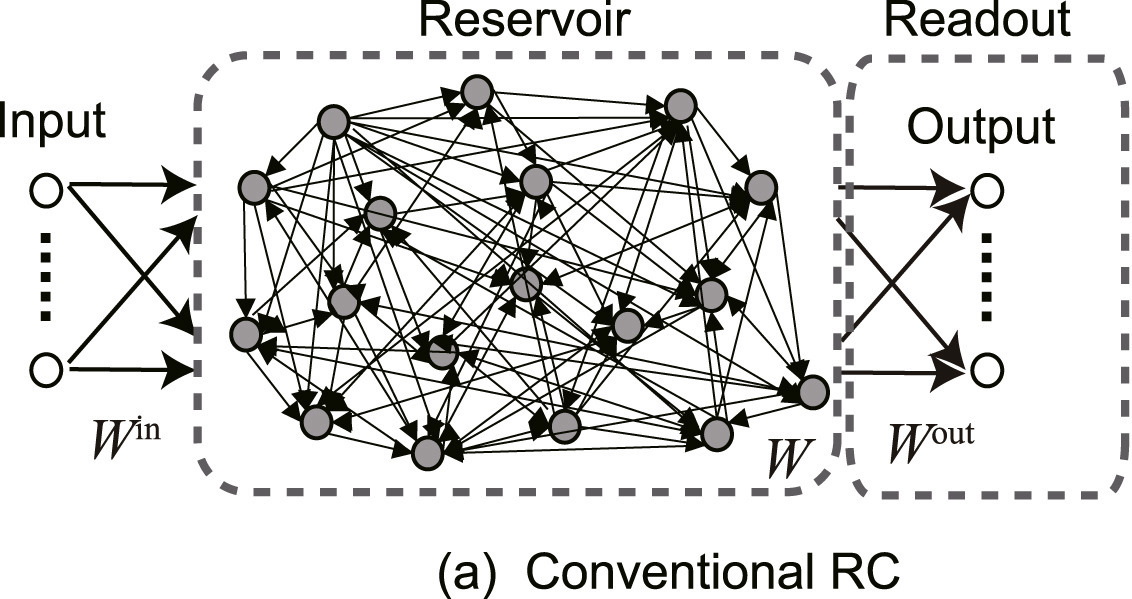
\includegraphics[width=0.99\textwidth]{reservoir}
    \caption[Structure of a Echo State Network]{Structure of a Echo State Network. The image is from \citeay{Tanaka_Yamane_Héroux_Nakane_Kanazawa_Takeda_Numata_Nakano_Hirose_2019}.}
    \figlbl{reservoir}
\end{figure}

The reservoir consists of \(N\) nodes which are connected according a Erdős–Rényi graph model\sidenote{The Erdős–Rényi model is a model for generating random graphs where all graphs on a fixed set of vertices and edges is equally likely} \sidecite{erdos59a}.
This graph model is represented by an adjacency matrix \(\boldsymbol{w}\)\sidenote{Figure \figref*{reservoir} uses upper case letter \(\boldsymbol{W}\)} of size \(N \times N\).
The time varying input signal \(\boldsymbol{x(t)}\) is mapped to a sub-set of \(N/M\) graph nodes by multiplying it with \(\boldsymbol{w}_{\text{in}} \in \mathbb{R}^{N\times M}\) and the output by multiplying the reservoir state with \(\boldsymbol{w}_{\text{out}} \in \mathbb{R}^{M\times N}\).
We refer interested reads to \sidecite{Lukoševičius_2012} to read more about the mathematical properties and how network is updated in detail.

In the original form of ESN, only the readout weights are learned, the rest is chosen randomly.
The input \(\boldsymbol{x(t)}\) brings the recurrent units in a initial state.
The recurrent connections inside the reservoir create different dynamics in the network.
The readout neurons linearly transform the recurrent dynamics into temporal outputs.
The readout weights \(\boldsymbol{w}_{\text{out}}\) are trained to reproduce a target function \(\boldsymbol{y(t)}\).

Liquid State machines use a spiking neural network instead of a graph of recurrent units as reservoir.
The nodes of the spiking neural network are randomly connected together.
Thus, every node receives time varying inputs from the inputs as well as from other nodes.
The recurrent connections turns the varying input into a spatio-temporal pattern.
Similar to ESN, the spatio-temporal patterns of activation are read out by a linear layer.

In general, reservoirs are universal approximators and can approximate any non-linear function given there are enough neurons in the reservoir.
They generalize better and faster than equivalent MLP.
The main drawback of current systems is that cannot deal well with high-dimensional inputs such as images.





